\documentclass{article}
\usepackage{spikey}
\usepackage{amsmath}
\usepackage{mathrsfs}
\usepackage{amssymb}
\usepackage{soul}
\usepackage{float}
\usepackage{graphicx}
\usepackage{hyperref}
\usepackage{fancyhdr}
\usepackage{xcolor}
\usepackage{chngcntr}
\usepackage{centernot}
\usepackage[shortlabels]{enumitem}
\usepackage[margin=1truein]{geometry}
\usepackage{tkz-graph}
\usepackage{dsfont}
\usepackage{caption}
\usepackage{subcaption}

\usepackage{setspace}
\linespread{1.15}
\usepackage[margin=1truein]{geometry}

\counterwithin{equation}{section}
\counterwithin{figure}{section}

\title{ECO426H1 Market Design: Auctions and Matching Markets}
\author{Tianyu Du}
\date{\today}

\begin{document}
	\maketitle
	\tableofcontents
	
	\newpage
	
	\section{Preliminary: Auctions}
	\begin{definition}
		An \textbf{auction} is an \ul{informational environment} consisting of
		\begin{enumerate}[(i)]
			\item \textbf{Bidding format rules}: the form of the bids, which can be price only, multi-attribute, price and quantity, or quantity only;
			\item \textbf{Bidding process rules}: Closing/timing rules, available information, rules for bid improvements/counter-bids, closing conditions;
			\item \textbf{Price and allocation rules}: final prices, quantities, winners.
		\end{enumerate}
		Auctions are commonly referred to as a \ul{market mechanism} as well as a \ul{price discovery mechanism}
	\end{definition}
	
	\begin{definition}
		A \textbf{market mechanism} uses prices to determine allocations.
	\end{definition}

	\begin{definition}
		An auction is a \textbf{private value} auction if agents' valuations do not dependent on other buyers' valuations. Otherwise, the auction is called a \textbf{interdependent / common value} auction.
	\end{definition}
	
	\begin{assumption}
		In a \ul{private value auction}, we shall impose the following assumption on bidders' valuations:
		\begin{enumerate}[(i)]
			\item Each bidder's valuation is independently and identically distributed on some interval $[0, \omega]$ according to a distribution function $F$:
			\begin{align}
				V_i \overset{i.i.d.}{\sim} F\ s.t.\ \tx{supp}(F) = \R_+
			\end{align}
			\item $F$ belongs to the common knowledge in this system;
			\item Bidders' valuations have finite expectations:
			\begin{align}
				\expect{V_i} < \infty
			\end{align}
		\end{enumerate}
	\end{assumption}
	
	\begin{assumption}
		Moreover, we assume bidders' behaviours to satisfy the following properties:
		\begin{enumerate}[(i)]
			\item Bidders are risk neutral, they are maximizing expected profits;
			\item Each bidder it both willing and able to pay up to his or her value.
		\end{enumerate}
	\end{assumption}
	
	\begin{definition}
		A \textbf{strategy} of a bidder is a mapping from the space of his/her valuation to a bid:
		\begin{align}
			s: [0, \omega] \to \R_+
		\end{align}
	\end{definition}
	
	\begin{definition}
		An equilibrium of auction is \textbf{symmetric} if all bidders are following the same bidding strategy $s$.
	\end{definition}
	
	\begin{definition}
		A bidder is \textbf{bidding sincerely / truthfully} if he bids his true value. 
	\end{definition}

	\begin{definition}
		An asymmetric game where played have private information is said to be \textbf{strategy proof}  if it is a weakly-dominant strategy for every player to reveal his/her private information.
	\end{definition}

	\begin{definition}
		An auction selling one item is a \textbf{standard auction} if the bidder with highest value is always the winner. That is, a standard auction maximizes social value.
	\end{definition}

	\section{Ascending Auctions: Extensive Form Games}
	
	\begin{definition}
		In an \textbf{English outcry auction}, bidders announce the prices,
		\begin{enumerate}[(i)]
			\item Bidders announce prices,
			\item with minimum increment between two bids (i.e., the ticking price).
			\item The auction ends when there's no further bid or when a time limit is reached.
			\item The winner is the one bidding the highest price.
			\item The winner pays his bid.
		\end{enumerate}
	\end{definition}
	
	\begin{remark}
		Bidding speed matters in English outcry auctions: two bidders cannot announce the same bid at the same time. 
	\end{remark}
	
	\begin{definition}
		In an \textbf{English auction / Japanese button auction},
		\begin{enumerate}[(i)]
			\item The auctioneer announces prices, the price goes up by the ticking price each round;
			\item in each round, bidders who feel this price is acceptable remain active, other bidders become inactive;
			\item bidders cannot be reactivated.
			\item the auction ends when there's no active bidder.
			\item the winner is the last bidder becomes inactive, if there's a tie, winner is randomly chosen.
			\item the price paid is the last announce price (the price corresponds to no active bidder).
		\end{enumerate}
	\end{definition}
	
	\begin{remark}
		In an English auction, the winner is the one with \ul{the highest valuation}, but the price is that of \ul{the second highest valuation plus the ticking price}.
	\end{remark}
	
	\begin{remark}
		In the English auction, the auctioneer learns (at the end) the valuations of all bidders except the valuation of the highest bidder.
	\end{remark}

	\section{Second Price Sealed-Bid Auction with Private Values}
	\begin{definition}
		In the \textbf{Vickrey auction / second price sealed-bid auction},
		\begin{enumerate}[(i)]
			\item Buyers submit a sealed-bid;
			\item The winner is the one with the highest bid,
			\item the winner pays the 2nd highest bid.
		\end{enumerate}
	\end{definition}
	
	\begin{remark}
		The second price sealed-bid auction and an English auction with negligible ticking price generate the same outcome. \\
		However, second price auction is a strategic for game, but English auction is an extensive form game. They are not exactly identical.
	\end{remark}

	\begin{proposition}
		In a symmetric equilibrium of the \ul{second-price} auction, $s(v) = v$ is a weakly dominant strategy.
	\end{proposition}
	
	\begin{proof}
		For a fixed valuation $v_i \in [0, \omega]$ of bidder $i$. \\
		Let $p := \max_{j \neq i} b_j$ be highest bidding price by other bidders. \\
		Let $\pi_i(b, p)$ denote bidder $i$'s profit when bidding $b$ given the highest price from other bidders to be $p$. \\
		\textbf{Part 1:} consider another bidding $z_i < v_i$, the following cases are possible: 
		\begin{enumerate}[(i)]
			\item $v_i < p \implies z_i < v_i < p \implies \pi_i(v_i, p) = \pi_i(z_i, p) = 0$ (bidder $i$ losses anyway).
			\item $v_i = p \implies \pi_i(v_i, p) = \pi_i(z_i, p) = 0$ (bidder $i$ is indifferent).
			\item $v_i > p$:
			\begin{enumerate}
				\item $v_i > z_i > p \implies \pi_i(v_i, p) = \pi_i(z_i, p) = v_i - p$;
				\item $v_i > z_i = p \implies \pi_i(v_i, p) \geq \pi_i(z_i, p)$;
				\item $v_i > p > z_i \implies \pi_i(v_i, p) > \pi_i(z_i, p)$.
			\end{enumerate}
		\end{enumerate}
		Hence, bidding $v_i$ weakly dominates bidding any value below it. \\
		\textbf{Part 2}: for $z_i > v_i$, the argument is similar. \\
		Therefore, bidding $v_i$ weakly dominates bidding any other values.
	\end{proof}
	
	\begin{remark}
		Refer to the general $k^{th}$ price sealed-bid auction with private values for an alternative proof to this proposition.
	\end{remark}
	
	\section{First Price Sealed-Bid Auction with Private Values}
	\begin{notation}
		Let $\beta^K(v)$ denote the symmetric equilibrium strategy in a $k$-th price auction.
	\end{notation}
	
	\begin{remark}
		For every continuous distribution $F$, the probability for a tie to happen is zero. Therefore, we ignore the tie for now.
	\end{remark}
	
	\begin{definition}[First Price Auction]
	Let $N$ denote the set of bidders such that $|N| = n$. For each bidder $i \in N$, his valuation of the auctioned item $V_i$ follows some distribution $F$. Further assume that $V_i \perp V_j$ for every $i \neq j$. \\
	Let $W(b, v_i)$ denote the event that player $i$, who has valuation $v_i$, wins by bidding $b \in \R_+$, define 
	\begin{align}
		W(b, v_i) \iff b > \max_{j \neq i} b_j
	\end{align}
	The payoff (utility) of bidder $i$, who has valuation $v_i$, is
	\begin{align}
		U(b, v_i) = \begin{cases}
			v_i - b &\tx{ if } W(b, v_i) \\
			0 &\tx{ otherwise}
		\end{cases}
	\end{align}
	\end{definition}
	
	\subsection{Symmetric Equilibrium Behaviour}
	\par Consider a symmetric environment such that all bidders are using the same \ul{strictly increasing} strategy $s(\cdot)$ such that $s(\cdot)$ is invertible.
	\paragraph{Equilibrium Strategy}
	\begin{proposition}
		In a symmetric equilibrium of the first-price auction, equilibrium bidding strategies are given by
		\begin{align}
			s(v_i) = \expect{\max_{j \neq i} v_j | v_j \leq v_i}
		\end{align}
		which is the \ul{expected second highest valuation conditional on $v_i$ being the highest valuation.}
	\end{proposition}
	
	\begin{proof}
		Let $s(v)$ denote an equilibrium strategy.
		\begin{lemma}
			For any agent, bidding more than $s(\omega)$ can never be optimal. Bidding $b > s(\omega)$ makes this agent win for sure. In such case, bidding $b' \in (s(\omega), b)$ strictly dominates bidding $b$.
		\end{lemma}
		\begin{lemma}
			For any agent, $s(0) = 0$. Bidding any positive number would cause negative payoff with positive probability, and therefore, leads to a negative expected profit.
		\end{lemma}
		\begin{lemma}
			Because $s$ is monotonically increasing, therefore,
			\begin{align}
				\max_{j \neq i} s(v_j) = s(\max_{j \neq i} v_j)
			\end{align}
		\end{lemma}
		Let $p$ denote the highest price among all other $N-1$ bidders and let $F^{(N-1)}(x)$ denote the distribution of $p$. \\
		The expected profit of bidder $i$ by bidding an arbitrary $b \in \R_+$ is
		\begin{align}
			\pi_i(b, v_i) &= P(b > p) (v_i - s(v_i))
			+ P(b = p) (v_i - s(v_i))
			+ P(b < p) 0
		\end{align}
		Note that $b > p = s(\max_{j \neq i}v_j)$ if and only if $s^{-1}(b) > \max_{j \neq i}v_j$. It follows
		\begin{align}
			P(b > p) = P(\max_{j \neq i}v_j < s^{-1}(b)) = F^{(N-1)}(s^{-1}(b))
		\end{align}
		Therefore,
		\begin{align}
			\pi_i(b, v_i) = F^{(N-1)}(s^{-1}(b)) (v_i - b)
		\end{align}
		The first order condition implies
		\begin{align}
			\pd{\pi_i}{b} \pi_i (b, v_i) 
			&= \pd{\pi_i}{b} F^{N-1} (s^{-1}(b)) v_i - F^{N-1} (s^{-1}(b)) b \\
			&= f^{(N-1)}(s^{-1}(b)) \frac{v_i - b}{s'(v_i)}
			- F^{(N-1)}(s^{-1}(b)) = 0
		\end{align}
		For a symmetric equilibrium, all other bidders are following the same strategy $s$ so that $s(v_i) = b$, therefore, 
		\begin{align}
			f^{(N-1)}(s^{-1}(b)) \frac{v_i - b}{s'(v_i)}
			- F^{(N-1)}(s^{-1}(b)) = 0 \\
			\implies f^{(N-1)}(s^{-1}(b)) (v_i - b)
			- F^{(N-1)}(s^{-1}(b)) s'(v_i) = 0 \\
			\implies f^{(N-1)}(s^{-1}(b)) v_i = F^{(N-1)}(s^{-1}(b)) s'(v_i) + f^{(N-1)}(s^{-1}(b)) s(v_i) \\
			\implies f^{(N-1)}(v_i) v_i = \frac{d}{dv_i} \left[ F^{(N-1)}(v_i) s(v_i) \right] \\
			\implies \int_{0}^{v_i} f^{(N-1)}(y) y\ dy = F^{(N-1)}(v_i) s(v_i) - F^{(N-1)}(0) s(0) \\
			\implies F^{(N-1)}(v_i) s(v_i) = \int_{0}^{v_i} f^{(N-1)}(y) y\ dy \\
			\implies s(v_i) = \frac{1}{F^{(N-1)}(v_i)} \int_{0}^{v_i} f^{(N-1)}(y) y\ dy \\
			\implies s(v_i) = \expe \left[\max_{j \neq i} v_j \right|\left. \max_{j \neq i} v_j < v_i \right]
		\end{align}
	\end{proof}
	When $F = Unif(0, 1)$.
	\begin{align}
		\beta^I(v) = \frac{n-1}{n} v
	\end{align}
	
	\paragraph{Probability of Winning}
	\begin{align}
		P(W(b, v_i))
		&= P(b > \max_{j \neq i} s(v_j)) \\
		&= P(b > s(\max_{j \neq i} v_j)) \\
		&= P(\max_{j \neq i} v_j \leq s^{-1}(b))) \\
		&= F(s^{-1}(b))^{n-1} \\
		&= F(v_i)^{n-1} \tx{ because } b = s(v_i)
	\end{align}
	When $F = Unif(0, 1)$,
	\begin{align}
		P(W(b, v_i)) &= v_i^{n-1}
	\end{align} 
	
	\paragraph{Expected Payment from Bidder $i$ with $v_i$ Conditioned on Winning} Suppose bidder $i$ is following strategy $s(\cdot)$. Then,
	\begin{align}
		\expect{Payment_i|v_i, W(b, v_i)} = b = s(v_i)
	\end{align}
	When $F = Unif(0, 1)$,
	\begin{align}
		\expect{Payment_i|v_i, W(b, v_i)} = \frac{n-1}{n} v_i
	\end{align}
	
	\paragraph{Unconditional Payment from Bidder $i$ with $v_i$}
	\begin{align}
		\expect{Payment_i|v_i} &= P(W(b, v_i)) \expect{Payment_i|v_i, W(b, v_i)} + P(Loss) \times 0 \\
		&= P(W(b, v_i)) \expect{Payment_i|v_i, W(b, v_i)} \\
		&= F(v_i)^{n-1} s(v_i)
	\end{align}
	When $F = Unif(0, 1)$,
	\begin{align}
		\expect{Payment_i|v_i} &= \frac{n-1}{n}v_i^n
	\end{align}

	\paragraph{Expected Payoff of Bidder $i$ with $v_i$}
	\begin{align}
		\expect{U|v_i}
		&= P(W(s(v_i), v_i)) v_i - \expect{Payment_i|v_i} \\
		&= F(v_i)^{n-1} v_i - F(v_i)^{n-1}s(v_i) \\
		&= F(v_i)^{n-1} [v_i - s(v_i)]
	\end{align}
	When $F = Unif(0, 1)$,
	\begin{align}
		\expect{U|v_i} = \frac{v_i^n}{n}
	\end{align}
	
	\paragraph{Unconditional Payment from Bidder $i$} This is the same as the expected revenue from bidder $i$:
	\begin{align}
		\expe [Payment_i] &= \int_{\R_+} \expect{Payment_i|v_i} dF \\
		&= \int_{\R_+} F(v_i)^{n-1} s(v_i) f(v_i)\ dv_i
	\end{align}
	When $F = Unif(0, 1)$,
	\begin{align}
		\expe [Payment_i] &= \int_0^1 \frac{n-1}{n}v_i^n\ dv_i \\
		&= \frac{n-1}{n(n+1)}
	\end{align}
	
	\paragraph{Auctioneer's Expected Revenue} Since all bidders are the same,
	\begin{align}
		\expect{Revenue} &= n\ \expe [Payment_i] \\
		&= n\ \int_{\R_+} F(v_i)^{n-1} s(v_i) f_i\ dv_i
	\end{align}
	When $F = Unif(0, 1)$,
	\begin{align}
		\expect{Revenue} = \frac{n-1}{n+1}
	\end{align}
	
	\section{Generalization: $k^{th}$ Price Sealed Bid Private Value Auction}
	\subsection{Uniform Values}
	\paragraph{} In a $k^{th}$ price auction, the bidder with the highest bidding wins, and pays the $k^{th}$ highest bid. Let $n$ denote the number of bidders.
	\begin{proposition}
		Assume $v_i \overset{i.i.d.}{\sim} Unif(0, 1)$, the following strategy forms a symmetric equilibrium in $k^{th}$ price auction:
		\begin{align}
			\red{\beta^{k}(v) = \frac{n-1}{n-k+1}v}
		\end{align}
	\end{proposition}
	
	\begin{proof}
		We are going to verify the proposed strategy indeed forms an equilibrium. \\
		Assume the optimal strategy is linear in $v$, say $\alpha v$ with $\alpha \in [0, 1]$, and all bidders other than $i$ are following this strategy. \\
		The expected payoff of bidder $i$ with value $v_i$ from bidding $b$ is
		\begin{align}
			U(b, v_i) &= \expe P(W(b, v_i)) (v_i - b_{n:k}) \\
			&= \expe P(b \geq \alpha v_j\ \forall j \neq i) (v_i - b_{n:k}) \\
			&= \expe P\left(v_j \leq \frac{b}{\alpha}\right)^{n-1} (v_i - b_{n:k}) \\
			&= \left(\frac{b}{\alpha}\right)^{n-1} v_i  - \left(\frac{b}{\alpha}\right)^{n-1} \expect{b_{n:k}|v_j \leq \frac{b}{\alpha}\ \forall j \neq i} \\
			&= \left(\frac{b}{\alpha}\right)^{n-1} v_i  - \left(\frac{b}{\alpha}\right)^{n-1} \alpha \expect{v_{n-1:k-1}|v_j \leq \frac{b}{\alpha}\ \forall j \neq i} \\
			&= \left(\frac{b}{\alpha}\right)^{n-1} v_i  - \left(\frac{b}{\alpha}\right)^{n-1} b \expect{v_{n-1:k-1}|v_j \leq 1\ \forall j \neq i} \\
			&= \left(\frac{b}{\alpha}\right)^{n-1} v_i  - \left(\frac{b}{\alpha}\right)^{n-1} b \expect{v_{n-1:k-1}} \\
		\end{align}
		Note that each individual $v_j \sim Unif(0, 1)$ for every $j$.\\
		The density function of $v_{n-1:k-1}$ is
		\begin{align}
			f_{v_{n-1:k-1}}(x)
			&= (n-1) \binom{n-2}{k-2} F(x)^{n-k} (1-F(x))^{k-2} f(x) \\
			&= (n-1) \binom{n-2}{k-2} x^{n-k} (1-x)^{k-2}
		\end{align}
		Taking the expectation
		\begin{align}
			\expect{v_{n-1:k-1}} &= \int_0^1 x f_{v_{n-1:k-1}}(x)\ dx \\
			&=  (n-1) \binom{n-2}{k-2} \int_0^1 x^{n-k+1} (1-x)^{k-2}\ dx \\
			&= (n-1) \binom{n-2}{k-2} \frac{\Gamma (k-1) \Gamma (-k+n+2)}{\Gamma (n+1)} \\
			&= \frac{-k+n+1}{n}
		\end{align}
		Therefore,
		\begin{align}
			U(b, v_i) &= \left(\frac{b}{\alpha}\right)^{n-1} \left(
			v_i - b \frac{-k+n+1}{n}
			\right)
		\end{align}
		
		\begin{proposition}
			Let $X_i \overset{i.i.d.}{\sim} Unif(0, 1)$ for $i = 1, \cdots n$, then
			\begin{align}
				\red{\expect{X_{n:k}} = \frac{n-k+1}{n+1}}
			\end{align}
		\end{proposition}
		
		Taking the first order condition,
		\begin{align}
			\pd{}{b} U(b, v_i) &= \frac{1}{\alpha^{n-1}}
			\pd{}{b} \left(
			b^{n-1} \left(
			v_i - b \frac{-k+n+1}{n}
			\right)
			\right) = 0 \\
			\implies
			&(n-1)b^{n-2}
			\left(
			v_i - b \frac{-k+n+1}{n}
			\right)
			- \frac{-k+n+1}{n} b^{n-1} = 0 \\
			\implies
			&(n-1)
			\left(
			v_i - b \frac{-k+n+1}{n}
			\right)
			- \frac{-k+n+1}{n} b = 0 \\
			\implies
			&(n-1)
			v_i - (n-1) b \frac{-k+n+1}{n}
			- \frac{-k+n+1}{n} b = 0 \\
			\implies &(n-1)v_i = (n-k+1)b \\
			\implies &\beta^K(v_i) = \frac{n-1}{n-k+1}
		\end{align}
	\end{proof}
	
	\paragraph{Probability of Winning Given $v_i$}
	\begin{align}
		P(W(s(v_i), v_i)) &= v_i^{n-1}
	\end{align}
	
	\paragraph{Probability of Payment Given $v_i$ Conditioned on Winning} Given that $v_i$ is the highest value, the payment conditioned on winning is
	\begin{align}
		\expect{s(v_{n-1:k-1})|v_j \leq v_i\ \forall j \neq i}
	\end{align}
	
	\section{Dutch/Descending Price Auction: An Extensive Form Game}
	\begin{definition}
		The \textbf{Dutch/descending price} auction is a first-price auction:
		\begin{enumerate}[(i)]
			\item There is a price clock: displays a price that is decreasing.
			\item The auction stops as soon as someone accepts the price.
			\item The first bidder accepts is the winner, and the price paid is exactly the last price displayed.
		\end{enumerate}
	\end{definition}

	\begin{remark}
		Dutch auction and first-price auction are equivalent, bidders use the same strategy, they have the same payoffs, and the auctioneer gets the same revenue.
	\end{remark}
	
	\section{Revenue Equivalence Theorem}
	\begin{theorem}
		For an auction with $n$ bidders. Suppose that values are independently and identically distributed and all bidders are risk-neutral. Then any symmetric and increasing equilibrium of any auction such that
		\begin{enumerate}[(i)]
			\item The winner is always the bidder with the highest valuation (i.e., standard auction);
			\item the bidder with the lowest valuation, $v_*$ has the same expected payoff $U_i(v_*)$ for all $i$,
		\end{enumerate}
		yields \ul{the same expected revenue} for the seller, and \ul{the same expected price} for any bidder in equilibrium.
	\end{theorem}
	
	\begin{proof}
		The expected payoff in equilibrium of someone with value $v_i$ is
		\begin{align}
			U_i(v_i) &= v_i P_w(v_i) - \expect{Payment_i} \\
			&= v_i P(v_i \geq v_j\ \forall j \neq i) - \expect{Payment_i}
		\end{align}
		Note that $v_i P(v_i \geq v_j\ \forall j \neq i)$ is independent from the auction format. \\
		Consider the case when the bidder is bidding $\beta(\tilde{v})$ instead of $\beta(v_i)$, that is, bidder $i$ is pretending to have another valuation,
		\begin{align}
			U_i(\tilde{v}, v_i) &= v_i P_w(\tilde{v}) - \expect{Payment_i} \\
			&= v_i P_w(\tilde{v}) - \expect{Payment_i} + \tilde{v}P_w(\tilde{v}) - \tilde{v}P_w(\tilde{v}) \\
			&= U_i(\tilde{v}) + P_w(\tilde{v})(v_i - \tilde{v})
		\end{align}
		Therefore,
		\begin{align}
			U_i(v_i) &\geq U_i(\tilde{v}, v_i) \\
			&= U_i(\tilde{v}) + P_w(\tilde{v})(v_i - \tilde{v}) \\
			\implies P_w(\tilde{v}) &\leq \frac{U_i(v_i) - U_i(\tilde{v})}{v_i - \tilde{v}}
		\end{align}
		Similarly, the same argument holds: someone with value $\tilde{v}$ won't deviate to behave like another $v_i$ value bidder.
		\begin{align}
			U_i(\tilde{v}) &\geq U_i(v_i, \tilde{v}) \\
			&= U_i(v_i) + P_w(v_i) (\tilde{v} - v_i) \\
			\implies P_w(v_i) &\geq \frac{U_i(v_i)- U_i(\tilde{v})}{v_i - \tilde{v}}
		\end{align}
		Hence, by taking the limit $\tilde{v} \to v_i$:
		\begin{align}
			\frac{dU_i(v)}{dv} &= P_w(v) \\
			\implies U_i(v_i) &= U_i(v_*) + \int_{v_*}^{v_i} P_w(v)\ dv 
		\end{align}
		Since $U_i(v_i)$ is independent from the auction format as well, therefore, the expected payment from bidder $i$ is independent from the auction format. Hence, the expected revenue of the auctioneer is 
		\begin{align}
			n \times \expect{Payment_i}
		\end{align}
		which is independent from the auction format as well.
	\end{proof}
	
	\section{Reserve Price \& Optimal Auctions}
	\par Let $r$ denote the reserve price, and $b_1, b_2$ denote the highest and second highest bid respectively. Then
	\begin{align}
		\text { Seller's revenue }=\left\{\begin{array}{ll}
		{0} & {\text { if } b_{1}<r} \\
		{r} & {\text { if } b_{2} \leq r \leq b_{1}} \\
		{b_{2}} & {\text { if } r<b_{2}}
		\end{array}\right.
	\end{align}
	
	\begin{definition}
		An \textbf{optimal auction} is an auction that maximizes the seller's revenue.
	\end{definition}
	
	\begin{theorem}[Myerson (1981), Riley \& Samuelson (1981)]
		If bidders' valuations are drawn independently from a distribution $F$, then a seller's \ul{optimal auction} is a  second-price auction with reserve price $r$ such that
		\begin{align}
			\psi(r) \equiv r - \frac{1 - F(r)}{f(r)} = 0
		\end{align}
	\end{theorem}
	
	\begin{proof}
		Note that this proof is extremely informal. \\
		The expected revenue can be written as (as if there is only one bidder):
		\begin{align}
			\expect{Revenue}
			&= P(v \leq r) 0 + P(v > r) r \\
			&= (1 - F(r)) r
		\end{align}
		Taking the first order condition
		\begin{align}
			(1 - F(r)) - r f(r) &= 0 \\
			\implies r - \frac{1 - F(r)}{f(r)} &= 0
		\end{align}
	\end{proof}
	
	\begin{remark}
		The theorem is applicable only if the auctioneer knows the exact distribution of bidders' values. In general, the auctioneer may know bidders' values are independently and identically distributed following some distribution, but not necessarily knows the exact form of this distribution.
	\end{remark}
	
	\begin{theorem}[Bulow \& Klemperer, 1996]
		When valuations are \ul{private} and \ul{independent}, a second-price auction with $n+1$ bidders gives a higher expected revenue than an optimal mechanism with $n$ bidders.
	\end{theorem}
	
	\begin{remark}
		The auctioneer is better off by bringing one additional bidder than by setting an optimal reserve price following the previous theorem.
	\end{remark}
	
	\begin{definition}
		A \textbf{Kirkegaard auction} is a two step auction:
		\begin{enumerate}[(i)]
			\item Run a second-price auction with $n$ bidders and \ul{optimal reserve price}. If the object isn't sold go to step 2.
			\item Sell the object for \$0 to $n+1$-th bidder.
		\end{enumerate}
		Obviously, this auction with $n+1$ bidders generates the same expected revenue as optimal $n$-auction (by setting the optimal reserve price).
	\end{definition}

	\begin{definition}
		An auction is \textbf{constrained optimal} if it maximizes the revenue among all auctions \ul{such that the object sold with certainty}.
	\end{definition}
	
	\begin{proof}[Proof. to Bulow \& Klemperer, 1996]
		Note that English auction with $n+1$ bidders is constrained optimal, therefore
		\begin{align}
			\expect{\tx{Optimal $n$ auction}} &= \expect{\tx{Kirkegaard  $n+1$}} \\
			&\leq \expect{\tx{English  $n+1$}}
		\end{align}
	\end{proof}
	
	\begin{corollary}
		The seller's expected revenue is the same for the English, Dutch, second-price and first-price auctions.
	\end{corollary}
	
	\section{Common Value Auction}
	\begin{definition}
		In a \textbf{common value} auction, all bidders' valuation are identical. However, bidders are receive \ul{private signals} $s_i$ provides information on the actual value $v$. Each bidder chooses a strategy $\beta_i(s_i) \in \R_+$ for all possible types of signals could be received. \\
		Specifically, bidders share a prior belief on the common value $v$ 
		\begin{align}
			v \sim p(v)	
		\end{align}
		and private signals are from the same distribution depends on the actual value $v$
		\begin{align}
			s_i \overset{i.i.d.}{\sim} p(s|v)
		\end{align}
	\end{definition}
	
	\begin{figure}[H]
		\centering
		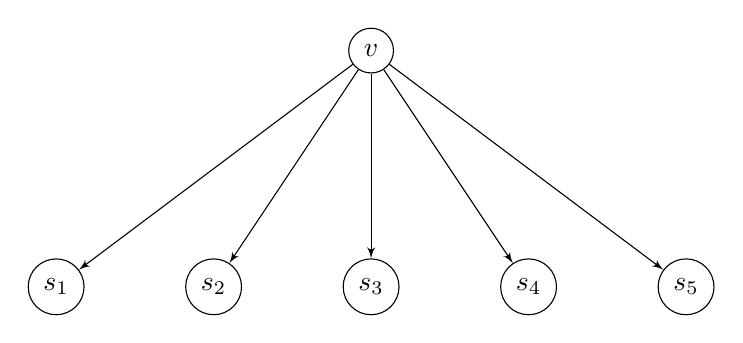
\begin{tikzpicture}
		\tikzset{vertex/.style = {shape=circle,draw,minimum size=1.5em}}
		\tikzset{edge/.style = {->,> = latex'}}
		\node[vertex] (v) at (5, 3) {$v$};
		\node[vertex] (s1) at (1, 0) {$s_1$};
		\node[vertex] (s2) at (3, 0) {$s_2$};
		\node[vertex] (s3) at (5, 0) {$s_3$};
		\node[vertex] (s4) at (7, 0) {$s_4$};
		\node[vertex] (s5) at (9, 0) {$s_5$};
		
		\draw[edge] (v) to (s1);
		\draw[edge] (v) to (s2);
		\draw[edge] (v) to (s3);
		\draw[edge] (v) to (s4);
		\draw[edge] (v) to (s5);
		\end{tikzpicture}
		\caption{DAG representation of common value auction with 5 bidders}
	\end{figure}

	\begin{example}
		Possible types of signals are
		\begin{align}
			s_i \overset{i.i.d.}{\sim} F\\ v = \sum_{i=1}^n s_i
		\end{align}
		or 
		\begin{align}
			s_i &= v + \varepsilon_i \\
			&\varepsilon_i \overset{i.i.d.}{\sim} Q\ s.t.\ \expect{\varepsilon_i} = 0
		\end{align}
	\end{example}
	\par In most cases, $v$ is positively correlated with the signal $s_i$ received by each bidder. That is,
	\begin{align}
		\pd{}{d s_j} \expect{v|s_1, \cdots, s_n} \geq 0\ \forall j \in N
	\end{align}
	Hence, we can assume bidding strategy $\beta$ to be an increasing function of signal $s$.
	
	\par In a common value auction, all bidders know the underlying random process generating $v$. Given $s_i$, bidder $i$ computes his \textbf{own estimation} of the common value $v$:
	\begin{align}
		v_i := \expect{v|s_i} = \iint_{s_{-i}} p(v|s_{-i}) p(s_{-i})
	\end{align}
	
	\paragraph{Formally} let 
	\begin{align}
		\Omega_i := \{s_j\ s.t.\ j \neq i| s_j \leq s_i\ \forall j \neq i\} \subseteq \R^{n-1}
	\end{align}
	denote the collection of realizations of signal generation such that bidder $i$ wins the auction. \\
	When bidder $i$ is winning the bid, the expected value is
	\begin{align}
		\expe [v|s_j \leq s_i\ \forall j \neq i, s_i]
		&= \frac{1}{P(\Omega_i)}\iint_{\Omega_i} p(s_{-i}) \expect{v|s_i, s_{-i}}\ ds_{-i} \\
		&\leq \iint_{\R^{n-1}} p(s_{-i}) \expect{v|s_i, s_{-i}}\ ds_{-i} \\
		&= \expect{v|s_i} = v_i
	\end{align}
	where the last inequality holds because $\expect{v|s_i, s_{-i}}$ is increasing in each $s$. 
	\begin{definition}
		\textbf{Winner's curse} winning the object reduces how much you think it is worth.
		Similarly, for \textbf{loser's curse} losing the auction may increase how much you think it is worth.
	\end{definition}
	
	\begin{proposition}
		Bidding one's own estimation $\expect{v|s_i}$ is not dominant in common value auction.
	\end{proposition}
	
	\begin{proposition}
		Symmetric bidding strategies in a second price common value auction are given by
		\begin{align}
			\beta^*(s_i) = \expect{v|s_i, s_{-i} = s_i}
		\end{align}
		In which the bidder assumes all other bidders are receiving the same signal.
	\end{proposition}
	
	\begin{proof}
		\todo{.}
	\end{proof}
	
	\section{Combinatorial Auction: The VCG Mechanism}
	\begin{definition}
		A Vickrey-Clarke-Groves (VCG) auction consists of a set of items to be sold $X$. Each bidder $i \in N$ has a private \textbf{value} for each possible bundle of items:
		\begin{align}
			v_i: \mc{P}(X) \to \R
		\end{align}
		Each bidder submits a (sealed) \textbf{bidding} for every possible bundle of items:
		\begin{align}
			b_i: \mc{P}(X) \to \R
		\end{align}
		An \textbf{assignment} characterize the allocation of items to bidders:
		\begin{align}
			\mu: N \to \mc{P}(X)
		\end{align}
		such that no item is shared between two bidders:
		\begin{align}
			\mu(i) \cap \mu(j) = \varnothing\ \forall i \neq j
		\end{align}
		The \textbf{outcome} assignment seeks to maximize the \ul{social value}. \\
		Note that the auctioneer does not know $v_j$'s, this social value is computed based on biddings $b_j$ instead of bidders' actual values.
		\begin{align}
			\mu^* = \argmax_{\mu} \sum_{i \in N} b_i(\mu(i))
		\end{align}
		The \textbf{price} paid by bidder $i$ is the \ul{externality this bidder imposes on other bidders.}:
		\begin{align}
			p_i = \max_\mu \sum_{j \neq i} b_j(\mu(j)) - \sum_{j \neq i}b_j(\mu^*(j))
		\end{align}
	\end{definition}
	
	\begin{remark}
		The auctioneer does not have to allocate all items in $X$, that is, $\mu$ is not necessary a partition of $X$. $\bigcup_{i \in N}\mu(i)$ is not necessary $X$.
	\end{remark}
	
	\begin{remark}
		When $|X| = 1$, VCG mechanism is the second price auction.
	\end{remark}
	
	\begin{proposition}
		Submitting one's true valuation function (i.e., $b_i = v_i$) is a dominate strategy in the VCG auction, that is, VCG auction is strategy proof.
	\end{proposition}
	
	\begin{proof}
		Suppose all other bidders are bidding $b_j$. \\
		Let $\mu^*$ be the allocation when bidder $i$ bid $b_i = v_i$ while all other bidders bid $b_j$:
		\begin{align}
			\mu^* = \argmax_\mu v_i(\mu(i)) + \sum_{j\neq i} b_j(\mu(j))\quad (\dagger)
		\end{align}
		Then, for bidder $i$, the payoff by bidding $v_i$ is
		\begin{align}
			v_i(\mu^*(i)) - \max_\mu \sum_{j \neq i} b_j(\mu(j)) + \sum_{j \neq i}b_j(\mu^*(j))
		\end{align}
		Alternatively, bidder $i$ could bid $b_i \neq v_i$, let
		\begin{align}
			\hat{\mu} = \argmax_\mu \sum_{i \in N} b_i(\mu_i(i))
		\end{align}
		The payoff from bidding $b_i$ instead is
		\begin{align}
			v_i(\hat{\mu}(i)) -  \max_\mu \sum_{j \neq i} b_j(\mu(j)) + \sum_{j \neq i}b_j(\hat{\mu}(j))
		\end{align}
		Take the difference between two payoffs:
		\begin{align}
			&v_i(\mu^*(i)) - \max_\mu \sum_{j \neq i} b_j(\mu(j)) + \sum_{j \neq i}b_j(\mu^*(j))
			- \left(
			v_i(\hat{\mu}(i)) -  \max_\mu \sum_{j \neq i} b_j(\mu(j)) + \sum_{j \neq i}b_j(\hat{\mu}(j))
			\right) \\
			&= v_i(\mu^*(i)) + \sum_{j \neq i}b_j(\mu^*(j)) - \left(v_i(\hat{\mu}(i)) + \sum_{j \neq i}b_j(\hat{\mu}(j))
			\right) \\
			&\geq 0 \tx{ by } (\dagger)
		\end{align}
		Therefore, bidding one's own value function is dominant.
	\end{proof}
	
	\begin{proposition}
		The price paid by any bidder in VCG auctions is non-negative.
	\end{proposition}
	
	\begin{proof}
		\begin{align}
			p_i = \max_\mu \sum_{j \neq i} b_j(\mu(j)) - \sum_{j \neq i}b_j(\mu^*(j)) \geq 0
		\end{align}
	\end{proof}
	
	\section{Keyword Auctions}
	
	\section{Two side, One-to-One Matching: Marriage Market}
	\begin{definition}[Marriage Market]
		Suppose there are a finite set of \textbf{women}: $W = \{w_1, w_2, \cdots\}$, and a finite set of \textbf{men}: $M = \{m_1, m_2, \cdots\}$. Each man $m \in M$ has a \ul{strict} preference relation $P_m$ over the women and the option of remaining single, that is, $P_m$ is defined over $W \cup \{m\}$. Similarly, each $w \in W$ has a preference relation $p_w$ over $M \cup \{w\}$.
	\end{definition}
	
	\begin{notation}
		The strict preference $P_v$ is often written as $\succ_v$. And the weak preference (i.e., preferred or indifferent to) is often written as $R_v$ or $\succsim_v$.
	\end{notation}
	
	\begin{definition}
		A man $m \in M$ is \textbf{unacceptable} for woman $w$ if and only if
		\begin{align}
			w P_w m
		\end{align}
	\end{definition}
	
	\begin{definition}
		A (one-to-one) \textbf{matching} is a mapping $\mu: W \cup M \to W \cup M$ such that
		\begin{itemize}
			\item $\forall m \in M,\ \mu(m) \in W \cup \{m\}$;
			\item $\forall w \in W,\ \mu(w) \in M \cup \{w\}$;
			\item $\mu(w) = m \iff \mu(m) = w$.
		\end{itemize}
	\end{definition}
	
	\begin{remark}
		Someone $v \in M \cup W$ is \textbf{unmatched} if $\mu(v) = v$.
	\end{remark}
	
	\begin{remark}
		There's no price in a matching problem, so we can't really talk about equilibrium.
	\end{remark}
	
	\begin{definition}
		A matching $\mu$ is \textbf{individually rational} if for each $v \in M \cup W$,
		\begin{align}
			\mu(v) \succsim_v v
		\end{align}
	\end{definition}
	
	\begin{definition}
		A pair $(m, w)$ \textbf{blocks} a matching $\mu$ if
		\begin{itemize}
			\item $\mu(m) \neq w$;
			\item $w \succsim_m \mu(m)$;
			\item $m \succsim_w \mu(w)$.
		\end{itemize}
	\end{definition}
	
	\begin{definition}
		A matching $\mu$ is \textbf{stable} if
		\begin{itemize}
			\item it is individually rational;
			\item and there is no $(m, w)$ pair blocks $\mu$.
		\end{itemize}
	\end{definition}
	
	\begin{theorem}[David Gale \& Lloyd Shapley, 1962]
		For any set of preferences, there always exists at least one stable matching.
	\end{theorem}
	
	\begin{algorithm}[Deferred Acceptance Algorithm] Man-proposing version:
		\begin{itemize}
			\item Step 1
			\begin{itemize}
				\item Each man proposes to his most preferred, acceptable woman (if a man finds no women acceptable he remains single);
				\item Each woman who received at least one offer (proposed):
				\begin{itemize}
					\item temporarily holds the offer from the most preferred man among those who made an offer to her and are acceptable,
					\item rejects all other offers.
				\end{itemize}
			\end{itemize}
			\item Step $k \geq 2$, each man whose offer has been rejected in the previous step proposes to his most preferred woman among the acceptable women he has not yet proposed to (if there is no such woman he remains single).
		\end{itemize}
		The algorithm stops when no rejection happens, and women are matched with their on-hold men.
	\end{algorithm}
	
	\begin{theorem}[David Gale \& Lloyd Shapley, 1962]
		For any set of preferences, there always exists at least one stable matching.
	\end{theorem}
	
%	\begin{proposition}
%		Let $\mu_M$ denote the man-proposing DA matching.
%		Each man prefers $\mu_M$ to any other stable matching.
%		Each woman prefers any stable matching to $\mu_M$.
%		Therefore, $\mu_M$ is the man-optimal matching.
%	\end{proposition}
%
%	\begin{proposition}
%		Let $\mu_W$ denote the woman-proposing DA matching.
%		Each woman prefers $\mu_W$ to any other stable matching.
%		Each man prefers any stable matching to $\mu_W$.
%		Therefore, $\mu_W$ is the woman-optimal matching.
%	\end{proposition}
	
	\begin{theorem}
		The Deferred Acceptance algorithm (DA) produces a stable matching that is
		\begin{itemize}
			\item The \ul{most preferred} stable matching for the \ul{proposing} side;
			\item The \ul{least preferred} stable matching for the \ul{receiving} side.
		\end{itemize}
	\end{theorem}
	
	\begin{proposition}
		A pair of man $m$ and women $m$ is \textbf{achievable} if there exists a \textbf{stable matching} $\mu$ such that $\mu(m) = w$.
	\end{proposition}
	
	\begin{proposition}
		Under man-proposing DA, no man can be rejected by an achievable woman.
	\end{proposition}
	
	\begin{proposition}
		Let $\mu$ and $\mu'$ be two stable matchings. Suppose all men weakly prefer $\mu$ to $\mu'$. Then all women must weakly prefer $\mu'$ to $\mu$.
	\end{proposition}
	
	\begin{theorem}
		A matching mechanism that uses the Deferred Acceptance algorithm is strategyproof for the \ul{proposing} side.
	\end{theorem}
	
	\begin{theorem}
		There is no matching mechanism that satisfies, for any matching problem, the following two properties at the same time:
		\begin{enumerate}[(a)]
			\item The matching is \ul{stable} with respect to the submitted preference lists;
			\item The mechanism is \ul{strategyproof} for \ul{all} individuals.
		\end{enumerate}
	\end{theorem}
	
	\section{Two side: Many-to-One Matching: Medical Matching}
	\begin{definition}[Medical Matching]
		The agents in this problem consist of a finite set of \textbf{doctors}(residents) and a finite set of \textbf{hospitals}:
	\begin{align}
		D &= \{d_1, d_2, \cdots \} \\
		H &= \{h_1, h_2, \cdots \}
	\end{align}
	For each $h \in H$, there is a \textbf{capacity} $q_h$ denotes the maximum number of residents $h$ can hire. And each $h \in H$ has a \ul{strict} preference over the set of doctors, $P_h^\sharp$. Note that $P_h^\sharp$ is only defined on sets with sizes up to $q_h$. \\
	For each $d \in D$, $d$ has a strict preference, $P_d$, over hospitals.
	\end{definition}
	
	\begin{definition}
		A preference relation $P_h^\sharp$ over $\mc{P}(D)$ is \textbf{responsive} if there exists another preference relation $P_h$ over $D$ such that: for every $S \subseteq D$ such that $|S| < q_h$, and any $d, d' \notin S$,
		\begin{align}
			S \cup \{d\} P_h^\sharp S \cup \{d'\} \iff d P_h d'
		\end{align}
		and
		\begin{align}
			S \cup \{d\} P_h^\sharp S \iff d \tx{ is acceptable to } h
		\end{align}
	\end{definition}

	\begin{definition}
		A \textbf{matching} is a function $\mu: U \cup D \to H \cup D$ such that
		\begin{itemize}
			\item $\forall d \in D,\ \mu(d) \in H \cup \{d\}$;
			\item $\forall h \in H$,
			\begin{itemize}
				\item $\abs{\mu(h)} \leq q_h$ (within capacity);
				\item $\mu(h) \subseteq D$ (only matched to doctors).
			\end{itemize}
			\item $\mu(d) = h \iff d \in \mu(h)$.
		\end{itemize}
	\end{definition}
	
	\begin{definition}
		A matching $\mu$ is \textbf{individually rational} if
		\begin{itemize}
			\item For each doctor $d \in D$, $\mu(d) \succsim_d d$.
			\item For each hospital $h \in H$, $\forall d \in \mu(h)$, $d \succsim_h \varnothing$.
		\end{itemize}
	\end{definition}
	
	\begin{definition}
		A pair $(d, h)$ \textbf{blocks} a matching $\mu$ if
		\begin{itemize}
			\item $d \notin \mu(h)$;
			\item $h P_d \mu(d)$;
			\item $d P_h d'$ for some $d' \in \mu(h)$.
		\end{itemize}
		Equivalently, with responsive preference:
		\begin{align}
			\mu(h) \cup \{d\} \backslash \{d'\} P_h^\sharp \mu(h)
		\end{align}
		That is, hospital $h$ would like to replace $d'$ with $d$.
	\end{definition}
	
	\begin{definition}
		A matching $\mu$ is \textbf{non-wasteful} if
		\begin{align}
			h P_d \mu(d) \implies \abs{\mu(h)} = q_h \lor \varnothing P_h d
		\end{align}
		If d prefers a hospital to her match then that hospital has filled its capacity (or d is not acceptable to h).
	\end{definition}
	
	\begin{definition}
		A matching $\mu$ is \textbf{stable} if
		\begin{itemize}
			\item it is individually rational;
			\item there is no blocking pair;
			\item it is non-wasteful.
		\end{itemize}
	\end{definition}
	
	\begin{algorithm}[Deferred Acceptance Algorithm for Many-to-One Matchings]
		Hospital-proposing version:
		\begin{itemize}
			\item Step 1
			\begin{itemize}
				\item Each hospital proposes to its most preferred \ul{set of doctors};
				\item Each doctor accepts the proposal/oer from their most preferred acceptable hospital, and rejects all other others.
			\end{itemize}
			\item Step $k \geq 2$, each hospital that had one or more rejections at the previous step proposes to its most preferred \ul{set of doctors} such that
			\begin{itemize}
				\item The set must contain all doctors that have accepted the hospital's offer at the previous step;
				\item Any additional doctor in the set must be a doctor to whom the hospital has not proposed to before.
			\end{itemize}
			Each doctor accepts the proposal/oer from their most preferred acceptable hospital, and rejects all other others.
		\end{itemize}
		The algorithm stops when \ul{no more offers are rejected}.
	\end{algorithm}
	
	\begin{proposition}
		Doctor proposing DA yields the doctor-optimal matching, Hospital proposing DA yields the hospital-optimal matching.
	\end{proposition}
	
	\begin{proposition}
		The doctor-proposing DA is strategyproof for doctors (but not for hospitals).
		However, the hospital proposing DA is \ul{not} strategyproof for hospitals.
	\end{proposition}
	
	\section{Kidney Exchange}

	\section{Appendix A: Order Statistics}
	\begin{definition}
		Let $(X_1, \cdots, X_n)$ be $n$ random variables on the probability space $(\Omega, \mc{F}, P)$, further assume they are iid following distribution function $F(\cdot)$. For each $\omega \in \Omega$, realizations of above random variables can be sorted as
		\begin{align}
			X_{(n)}(\omega) \leq X_{(n-1)}(\omega) \leq \cdots \leq X_{(1)}(\omega)
		\end{align}
		For each $\omega$, the random variable $X_{n:k}$ is defined such that $X_{n:k}(\omega)$ equals the $k$-th largest value, $X_{(k)}(\omega)$.
	\end{definition}
	
	\paragraph{Distribution Function} Let $x \in X(\Omega)$, then 
	\begin{align}
		X_{n:k} \leq x
		&\iff (\tx{no $X_i > x$}) \bigcup \left(\tx{exactly $1$ $X_i > x$}\right) \bigcup  \cdots \bigcup \left(\tx{exactly $k-1$ $X_i > x$}\right) \\
		&\iff (X_i \leq x\ \forall i) \bigcup \left(\tx{exactly $n-1$ $X_i \leq x$}\right) \bigcup  \cdots \bigcup \left(\tx{exactly $n-k+1$ $X_i \leq x$}\right) \\
		&\iff \bigcup_{j=n-k+1}^n \left(\tx{exactly $j$ $X_i \leq x$}\right)
	\end{align}
	Note that events in the union are mutually exclusive, therefore,
	\begin{align}
		F_{n:k}(x) = P(X_{n:k} \leq x)
		&= \sum_{j=n-k+1}^n P\left(\tx{exactly $j$ $X_i \leq x$}\right) \\
		&= \red{\sum_{j=n-k+1}^n \binom{n}{j} F(x)^j (1 - F(x))^{n-j}}
	\end{align}
	\paragraph{Density Function}
	\begin{align}
		f_{n:k}(x)
		&= \frac{d}{dx} F_{n:k}(x) \\
		&= \frac{d}{dx} \sum_{j=n-k+1}^n \binom{n}{j} F(x)^j (1 - F(x))^{n-j} \\
		&= \frac{d}{dx} \sum_{j=n-k+1}^n \frac{n!}{j!(n-j)!} F(x)^j (1 - F(x))^{n-j} \\
		&= \sum_{j=n-k+1}^n \left[
		\frac{n!}{j!(n-j)!} j F(x)^{j-1} (1 - F(x))^{n-j}
		- \frac{n!}{j!(n-j)!} (n-j) F(x)^j (1 - F(x))^{n-j-1}
		\right]f(x)\\
		&= \sum_{j=n-k+1}^n 
		\frac{n!}{j!(n-j)!} j F(x)^{j-1} (1 - F(x))^{n-j} f(x)
		- \sum_{j=n-k+1}^{n-1} 
		\frac{n!}{j!(n-j)!} (n-j) F(x)^j (1 - F(x))^{n-j-1} f(x)\\
		&= \sum_{j=n-k+1}^n
		\frac{n!}{(j-1)!(n-j)!} F(x)^{j-1} (1 - F(x))^{n-j} f(x)
		- \sum_{j=n-k+1}^{n-1}
		\frac{n!}{j!(n-j-1)!} F(x)^j (1 - F(x))^{n-j-1} f(x) \\
		&=\begin{aligned}[t]
			&\frac{n!}{(n-k)!(k-1)!} F(x)^{n-k} (1 - F(x))^{k-1} f(x) \\
			&+ \sum_{j=n-k+2}^n
			\frac{n!}{(j-1)!(n-j)!} F(x)^{j-1} (1 - F(x))^{n-j} f(x) \\
			&- \sum_{j=n-k+1}^{n-1}
			\frac{n!}{j!(n-j-1)!} F(x)^j (1 - F(x))^{n-j-1} f(x)
		\end{aligned} \\
		&=\begin{aligned}[t]
			&\frac{n!}{(n-k)!(k-1)!} F(x)^{n-k} (1 - F(x))^{k-1} f(x) \\
			&+ \sum_{j=n-k+2}^n
			\frac{n!}{(j-1)!(n-j)!} F(x)^{j-1} (1 - F(x))^{n-j} f(x) \\
			&- \sum_{i=n-k+2}^{n}
			\frac{n!}{(i-1)!(n-i)!} F(x)^{i-1} (1 - F(x))^{n-i} f(x) \text{ (substitute $j = i - 1$)}
		\end{aligned} \\
		&= \frac{n!}{(n-k)!(k-1)!} F(x)^{n-k} (1 - F(x))^{k-1} f(x) \\
		&= n \frac{(n-1)!}{(n-k)!(k-1)!} F(x)^{n-k} (1 - F(x))^{k-1} f(x) \\
		&= \red{
		n \binom{n-1}{k-1} F(x)^{n-k} (1 - F(x))^{k-1} f(x)
		}
	\end{align}
\end{document}























